\documentclass{standalone}
\usepackage{tikz}
\begin{document}
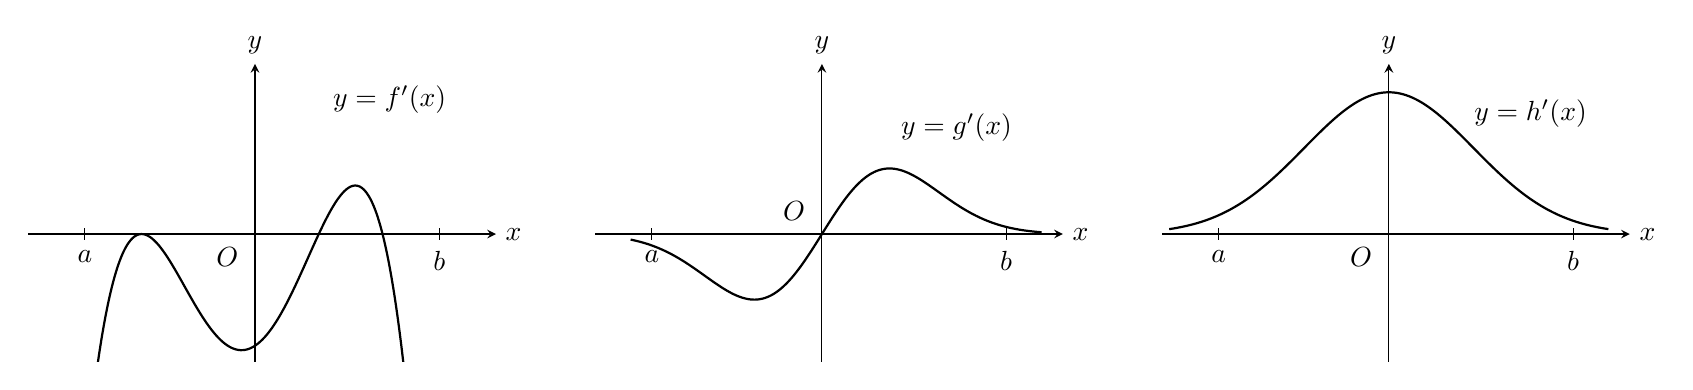
\begin{tikzpicture}[>=stealth, scale=0.9]

  %=====================================================================
  % Panel 1: y = f'(x)
  %=====================================================================
  \begin{scope}[xshift=0cm]
    % axes
    \draw[->] (-3.2,0) -- (3.4,0) node[right] {$x$};
    \draw[->] (0,-1.8) -- (0,2.4) node[above] {$y$};
    \node[anchor=north east] at (-0.1,-0.05) {$O$};
    % a and b tick labels
    \node[anchor=north] at (-2.4,-0.1) {$a$};
    \node[anchor=north] at (2.6,-0.1) {$b$};
    % small tick marks for a and b
    \draw (-2.4,0.08) -- (-2.4,-0.08);
    \draw (2.6,0.08) -- (2.6,-0.08);

    \begin{scope}
      \clip (-3.2,-1.8) rectangle (3.4,2.4);
      % quartic, negative leading coeff (opens downward):
      % double root at x=-1.6 (local max touching y=0, ~1/3 from a to O),
      % two more zeros at x=0.9 and x=1.8 (between O and b)
      \draw[thick] plot[smooth,domain=-3.1:3.1,samples=200]
        ({\x},{-0.38*(\x+1.6)*(\x+1.6)*(\x-0.9)*(\x-1.8)});
    \end{scope}
    \node at (1.9,1.9) {$y = f'(x)$};
  \end{scope}

  %=====================================================================
  % Panel 2: y = g'(x)
  %=====================================================================
  \begin{scope}[xshift=8cm]
    \draw[->] (-3.2,0) -- (3.4,0) node[right] {$x$};
    \draw[->] (0,-1.8) -- (0,2.4) node[above] {$y$};
    \node[anchor=south east] at (-0.1,0.05) {$O$};
    \node[anchor=north] at (-2.4,-0.1) {$a$};
    \node[anchor=north] at (2.6,-0.1) {$b$};
    \draw (-2.4,0.08) -- (-2.4,-0.08);
    \draw (2.6,0.08) -- (2.6,-0.08);

    \begin{scope}
      \clip (-3.2,-1.8) rectangle (3.4,2.4);
      % odd-ish S curve: cross near a, trough, up through O, small peak, decay toward b
      \draw[thick] plot[smooth,domain=-2.7:3.1,samples=200]
        ({\x},{1.6*\x*exp(-0.55*\x*\x)});
    \end{scope}
    \node at (1.9,1.5) {$y = g'(x)$};
  \end{scope}

  %=====================================================================
  % Panel 3: y = h'(x)
  %=====================================================================
  \begin{scope}[xshift=16cm]
    \draw[->] (-3.2,0) -- (3.4,0) node[right] {$x$};
    \draw[->] (0,-1.8) -- (0,2.4) node[above] {$y$};
    \node[anchor=north east] at (-0.1,-0.05) {$O$};
    \node[anchor=north] at (-2.4,-0.1) {$a$};
    \node[anchor=north] at (2.6,-0.1) {$b$};
    \draw (-2.4,0.08) -- (-2.4,-0.08);
    \draw (2.6,0.08) -- (2.6,-0.08);

    \begin{scope}
      \clip (-3.2,-1.8) rectangle (3.4,2.4);
      % bell-shaped curve centered at O
      \draw[thick] plot[smooth,domain=-3.1:3.1,samples=200]
        ({\x},{2.0*exp(-0.35*\x*\x)});
    \end{scope}
    \node at (2.0,1.7) {$y = h'(x)$};
  \end{scope}

\end{tikzpicture}
\end{document}
